\documentclass{article}
\usepackage[utf8]{inputenc}
\usepackage{graphicx}
\usepackage{amsmath}
\usepackage{float}
\usepackage{lscape}
\usepackage{subcaption} %Side by side images
\usepackage[a4paper, margin=3cm]{geometry}

% Fancy tables
\usepackage{booktabs}

% Code viewing
\usepackage{listings}
\usepackage{color}

% Table of contents control: 
\usepackage{setspace}

\definecolor{mygreen}{rgb}{0,0.6,0}
\definecolor{mygray}{rgb}{0.5,0.5,0.5}
\definecolor{mymauve}{rgb}{0.58,0,0.82}

\lstset{ 
  backgroundcolor=\color{white},   % choose the background color; you must add \usepackage{color} or \usepackage{xcolor}; should come as last argument
  basicstyle=\footnotesize,        % the size of the fonts that are used for the code
  breakatwhitespace=false,         % sets if automatic breaks should only happen at whitespace
  breaklines=true,                 % sets automatic line breaking
  captionpos=b,                    % sets the caption-position to bottom
  commentstyle=\color{mygreen},    % comment style
  deletekeywords={...},            % if you want to delete keywords from the given language
  escapeinside={\%*}{*)},          % if you want to add LaTeX within your code
  extendedchars=true,              % lets you use non-ASCII characters; for 8-bits encodings only, does not work with UTF-8
  firstnumber=1,                   % start line enumeration with line 1000
  frame=single,	                   % adds a frame around the code
  keepspaces=true,                 % keeps spaces in text, useful for keeping indentation of code (possibly needs columns=flexible)
  keywordstyle=\color{blue},       % keyword style
  language=Octave,                 % the language of the code
  morekeywords={*,...},            % if you want to add more keywords to the set
  numbers=left,                    % where to put the line-numbers; possible values are (none, left, right)
  numbersep=5pt,                   % how far the line-numbers are from the code
  numberstyle=\tiny\color{mygray}, % the style that is used for the line-numbers
  rulecolor=\color{black},         % if not set, the frame-color may be changed on line-breaks within not-black text (e.g. comments (green here))
  showspaces=false,                % show spaces everywhere adding particular underscores; it overrides 'showstringspaces'
  showstringspaces=false,          % underline spaces within strings only
  showtabs=false,                  % show tabs within strings adding particular underscores
  stepnumber=1,                    % the step between two line-numbers. If it's 1, each line will be numbered
  stringstyle=\color{mymauve},     % string literal style
  tabsize=2,	                   % sets default tabsize to 2 spaces
  title=\lstname                   % show the filename of files included with \lstinputlisting; also try caption instead of title
}


%User defined commands
\newcommand*\mean[1]{\overline{#1}}

\newcommand*\hadamarddiv{\obslash} %Hadamard division

\title{Project-thesis}
\author{Erik Rundhovde M\o renskog}
\date{September 2019}

% Document setup
\setlength{\parindent}{0em}
\setlength{\parskip}{1em}

\begin{document}

% Title page
\begin{titlepage}
    
    
\includegraphics[width=0.4\textwidth]{figures/ntnu_hovedlogo_eng_svart.png}
    
    \vspace{1cm}
    \huge
    
    \textbf{Project Thesis TFE4580}
 
    \vspace{0.5cm}
    
    Sensor Fusion \\ 
    Camera and Spectrometer
 
    \vspace{1.5cm}
    \Large
    
    \textbf{Erik Rundhovde M\o renskog}

    \vfill

    December 2019
    
    \vspace{0.5cm}

    Supervised by Harald Ian Muri and Dag Roar Hjelme
\end{titlepage}

\singlespacing
\tableofcontents

\section{Abstract}
The waste industry is in need of cheaper ways of analyzing waste. This paper will look into if it is feasible to sensor fuse camera and spectrometer as an alternative to hyperspectral cameras. This feasibility is tested by comparing average values that should be proportional too each other between the systems. If these values are proportional to each other it will make the calibration of camera to spectrometer easier. 

\section{Introduction}
Hyperspectral imaging is extremely useful for classifying substances from a distance, but it is also very expensive. This paper will study if it is possible to use the much cheaper combination of camera and spectrometer instead of a hyperspectral camera in ideal situations. 
Hyperspectral imaging is a growing technology for remote sensing. The advantage is that you can get high spectral resolution in combination with high spatial resolution, usually 1 dimension for each. The proposed alternative is one where a camera is combined with a spectrometer. The camera will be able to give high spatial resolution in 2D, while the spectrometer will provide high spectral information for the same sample. The theoretical setup is shown in figure \ref{fig:measurement_setup}. 

Postulate: 
The spatial average of each color across an image is comparable with the spectral average of a spectrum that has been multiplied with the quantum efficiency of the camera sensor. Postulates further that the relationship between the values can be found through linear regression. This will have the following uses: 
\begin{itemize}
    \item The regression line can be used to tell if an image and a specter is taken correctly, that they are watching the same object. 
    \item If the previous is known to be true the regression line can give information about noise, from ambient light or other sources. 
\end{itemize}

%TODO: Add the focus which is finding correlating values between camera and spectrometer

\begin{figure}[h]
    \centering
    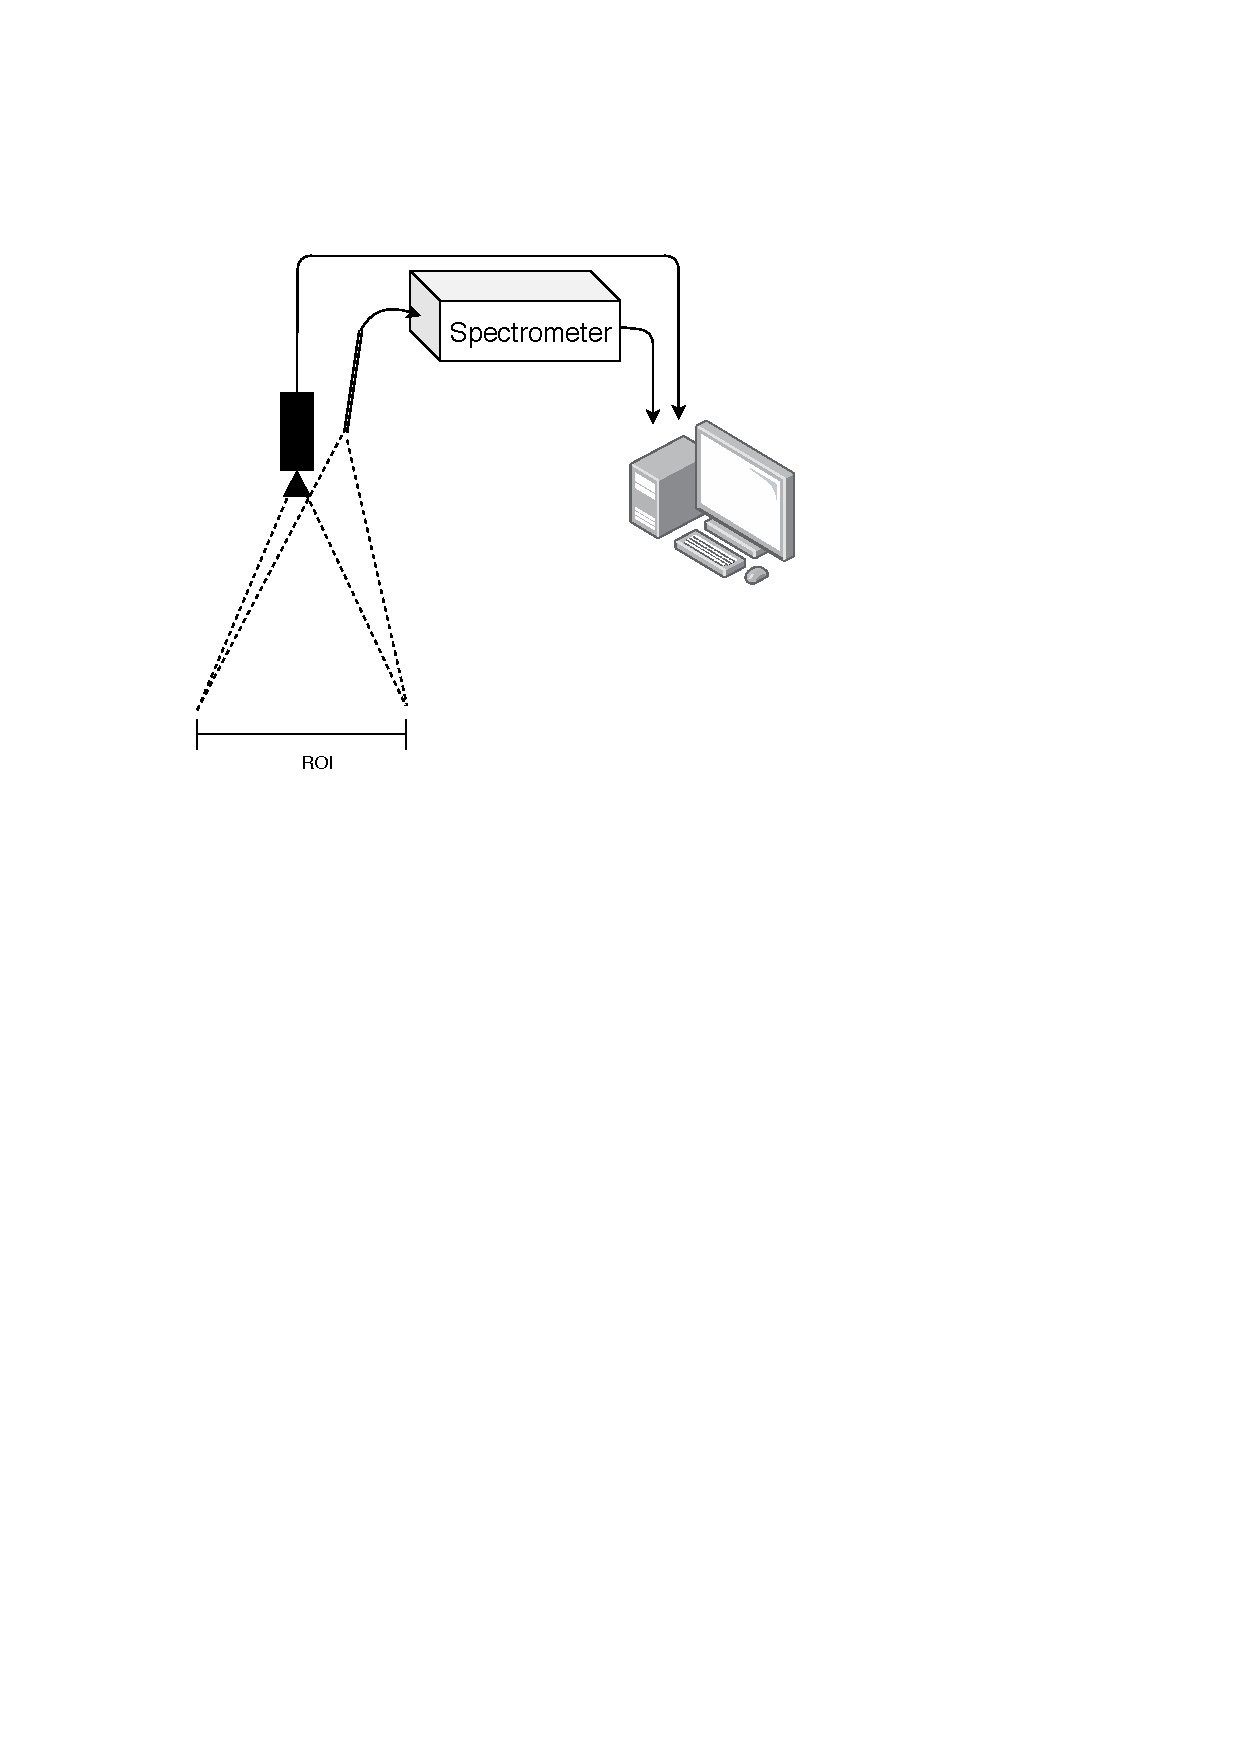
\includegraphics[width=0.5\textwidth]{figures/pt_setup.pdf}
    \caption{Measurement setup}
    \label{fig:measurement_setup}
\end{figure}



\section{Theory}
%TODO: Need theory about ccd? It is not really relevant is it?
%Need theory about the different uses of the same sensor in spectrometer and camera, I need this defend that the values should have an correlation. 

\subsection{Camera}
Cameras are widely used to photograph objects, and works by focusing light onto a photo-sensor. The camera used in this thesis uses a Charged-coupled device (CCD) photo-sensor \cite{JYIVolumeThree}.

\subsection{Spectrometry}
Spectrometer is a widely used tool for analyzing substances. It is a remote sensing tool that give good spectral information about the light that enters the fiber. As can be seen in figure \ref{fig:spectrometer_inside} the light is split into the different wavelengths before hitting the CCD sensor. This has the effect that the sensor reads spectral information instead of spatial as a camera would. 

\begin{figure}[h]
    \centering
    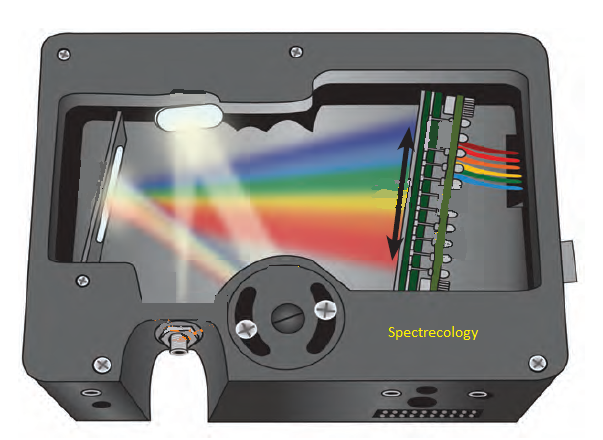
\includegraphics[width=0.5\textwidth]{figures/Mini-spectrometer-open-bench.png}
    \caption{Inside of a spectrometer \cite{KAI0340640480}}
    \label{fig:spectrometer_inside}
\end{figure}

Because of this it can be used to give an average spectrum of the area under the acceptance cone of the fiber. 
%TODO3 Add theory about how the spectrometer works. I could maybe skip this point as it is not necessary for explaining the correlation, but I'm afraid it is necessary for a rigorous description of why the correlation makes sense. Same for the camera

\subsection{Reflection}
\label{sec:theory_reflection}
Reflection of light describes the notion of light hitting materials and getting a change of path due to the exchange of energy with the material. There are two extremes when we talk about reflection:

\textbf{Specular reflection} denotes the case where the light is reflected in a unison manner from the sample, all in one direction. This concept is shown in figure \ref{fig:specular_reflection}.

\begin{figure}[h!]
    \centering
    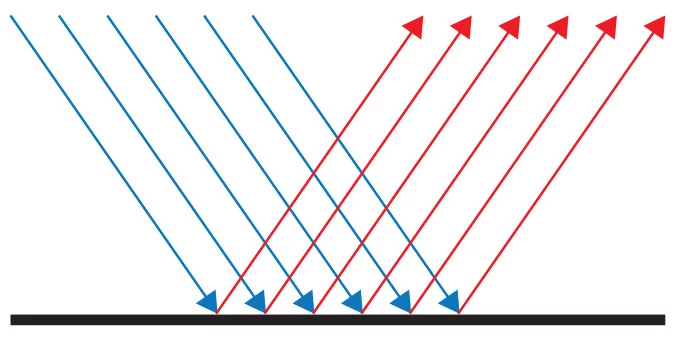
\includegraphics[width=0.5\textwidth]{figures/theory/Specular-Reflection.png}
    \caption{Example of specular reflection \cite{SpecularReflectionOcean}}
    \label{fig:specular_reflection}
\end{figure}

\textbf{Diffusive reflection} denotes the case where the light is scattered in every direction. This concept is shown in figure \ref{fig:diffusive_reflection}.

\begin{figure}[h!]
    \centering
    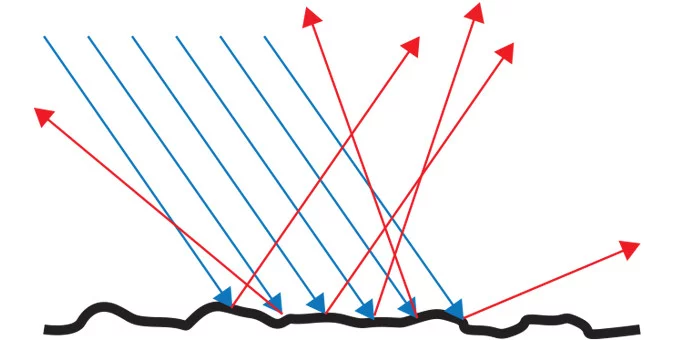
\includegraphics[width=0.5\textwidth]{figures/theory/Diffuse-Reflection.png}
    \caption{Example of diffusive reflection \cite{DiffuseReflectionOcean}}
    \label{fig:diffusive_reflection}
\end{figure}

Both of these reflection types are ideal and all real reflection will be a combination of these two. Not even the best available mirrors exhibit perfect specular properties, and no material scatters light equally in all directions. It is however useful to have two extremes to compare the results too. 

%TODO: Im not sure yet about including these
%\subsubsection{Specular} 
%\subsubsection{Diffusive}
%\subsection{Relative reflection}

\subsection{Noise and dark current}
\label{sec:noise_and_dark_current}
Both the images and the spectrums will have noise in them, making the readings less accurate. One type of noise that is a problem in spectrometry is noise from dark currents. These are currents that will be detected in the CCD sensor even though there is no incoming light. 



%TODO: Should add:
% Linear regression
% Colorimetry
% 

\section{Definitions}
This section will introduce all the math notation and equations that will be used in the paper. 

\subsection{Linear regression}
\label{sec:regression}
Linear regression is a technique to find the function of the form (\ref{eq:linear_function}) that have the minimum total square distance to the points in the set. 

\begin{equation}
    f(x) = ax + b
    \label{eq:linear_function}
\end{equation}


\subsection{Image}

Each pixel of the image will be described by a vector (\ref{eq:vector_pixel_bgr}), where each point on the vector describes one of the colors blue (B), green (G) and red (R).  This together gives the color combination of each pixel. Each color is an unsigned integers. 


\begin{equation}
    \label{eq:vector_pixel_bgr}
    \vec{p}_{ij} = [B,G,R]
\end{equation} 

One whole image will be stored in a matrix where each element of the matrix is a vector described by (\ref{eq:vector_pixel_bgr}). The matrix $A_{N\cdot M}$, where $N$ is the number of rows and $M$ is the number of columns, is shown in (\ref{eq:image_matrix})

\begin{equation}
    \label{eq:image_matrix}
    A = A_{N\cdot M} =  
    \begin{bmatrix}
        \vec{p}_{11} & \vec{p}_{12} & \cdots & & \vec{p}_{1M}  \\
        \vec{p}_{21} & \ddots &        &       &                \\
        \vdots       &        &\vec{p}_{ij}&   & \vdots          \\
                     &        &        & \ddots&                  \\
        \vec{p}_{N1} &        &        &       & \vec{p}_{NM}  
    \end{bmatrix}
\end{equation}

A second matrix to introduce is the special case where the image is the reference image, this special case will be denoted as $A_0$.

\subsubsection{Spatial average}
\label{sec:spatial_average}

An important equation later is the one that takes the spatial average of the matrix, this is done with (\ref{eq:spatial_sum}).
\begin{equation}
    \label{eq:spatial_sum}
    \mean{\vec{p}} = \frac{1}{NM} \sum_{i=0}^{N-1} \sum_{j=0}^{M-1} \vec{p}_{ij}
\end{equation}


\subsubsection{Hadamard division}
Element wise division will be used to compare two pictures, and is defined by the Hadamard division \cite{HadamardDivisionInfixed}:
\begin{equation}
    \label{eq:element_wise_division_image}
    A \oslash  A_0  \frac{A_{ij}}{A_{0ij} } %TODO
\end{equation}


\subsection{Spectrum}
\label{sec:spectrum}

The spectrum read from the spectrometer is saved in a $C x 2$ matrix, where $C$ is the dataset length, the first column is the wavelength ($\lambda$) and the second column is the corresponding intensity (\ref{eq:intensity})
\begin{equation}
    \label{eq:intensity}
    I = I(\lambda)    
\end{equation}

\begin{equation}
    \label{eq:intensity_0_background}
    I_0 = I_0(\lambda)
\end{equation}

We will also define a value (\ref{eq:intensity_0_background}) which is $I$ for the special case where the spectrum is muffin the background spectral response without any objects. From these definitions we define relative reflectance $RR$ (\ref{eq:relative_reflectance}). 

\begin{equation}
    \label{eq:relative_reflectance}
    RR = \frac{I}{I_0}
\end{equation}


The introduction of (\ref{eq:relative_reflectance_minus_one}) will make it easier see the changes in the spectrum when multiplying with QE.  
\begin{equation}
    \label{eq:relative_reflectance_minus_one}
    RR_2 = RR - 1
\end{equation}

We further introduce the notion of finding the spectrum corresponding to one color in the camera. Each pixel in the camera measures the light intensity for blue, green and red with a certain quantum efficiency given by the manufacturer. These values will be represented in a vector (\ref{eq:quantum_efficiency}) with three values corresponding to each wavelength $\lambda$. These values will represent how well each color is received by the camera and will be a float between zero and 1. 

\begin{equation}
    \label{eq:quantum_efficiency}
    \vec{QE}(\lambda)    
\end{equation}

This value can theoretically be used to relate the relative picture values with the relative reflectance values. This would be a major advantage as it can give us an insight into the noise factor affecting the sensor fusion.  

\subsubsection{Sectral average}
\label{sec:spectral_average}

The spectral equivalent of spatial sum (\ref{eq:spatial_sum}) is to take the integral of the graph and divide it by the wavelength range (\ref{eq:average_integral}). The trapezoidal rule was used to approximate the integral \cite{TrapezoidRuleMathematical}. 

\begin{equation}
    \label{eq:average_integral}
    \mean{\vec{RR}} = \frac{1}{\lambda_1 - \lambda_0} \int_{\lambda_0}^{\lambda_1} RR \cdot \vec{QE} \,\mathrm{d}\lambda 
\end{equation}


\subsubsection{Error function}
\label{sec:error_function}
To have an idea of how well an estimation works, an error function can be used. The function that will be used here takes the Euclidean distance between a data-point and the closest point in the estimation. The estimation will be a straight line in this setup, so the minimum distance between a point and the line can be found using the cross product. This function works by using three points, two of them should be points on the line ($p_0$ and $p_1$), and one should be the data point ($p$). The function is given in (\ref{eq:error_function}), where $\left\lVert .\right\rVert$ shows the second norm. 

\begin{equation}
    \label{eq:error_function}
    d = \frac{(p - p_0) \times (p_1 - p_0)}{\left\lVert p_1 - p_0\right\rVert _2}
\end{equation}

\section{Method}
Both the spectrums and the images will be analysed using spectrometer methods, this will open up for the opportunity to pre-process spectral and spatial data in the same way. We will then hopefully be able to compare the data more directly. The spectrometer processing method we want to use is relative reflectance ($RR$). Since this method is also being used with the spectrometer, it will be denoted $RR'$ whenever it is used for imaging. As can be seen from (\ref{eq:relative_reflectance}), relative reflectance is done by dividing the interesting values with a reference. The translation to image processing must be to divide every image pixel with a pixel value from a reference image. For comparing values with the spectrometer it is fully ok to do this division as long as the reference image is non-zero for all pixels. For that reason it is important with a well lit and preferably white background. 


One problem with this method is that images can only be visualized as three sets of integers between 0 and 255, i.e. the colors blue, green and red. Therefore we divide the division into to two cases when visualizing; reference divided by image and image divided by reference. The product will be denoted $RR'_{negative}$ for the reference divided by image case, and $RR'_{positive}$ for the image divided by reference case. The processing can be view in figure \ref{fig:image_visualization_program_flow}. Here $A$ is the image with an object and $A_0$ is the reference image. To deal with noise in the system, a noise limit is put in place before doing the division. This noise limit ensures that the difference between the image to be analysed and the reference is large enough to be assumed as a signal and not noise. This paper will later find the noise limit value with the infamous trial and error method. 

\begin{figure}[h]
    \centering
    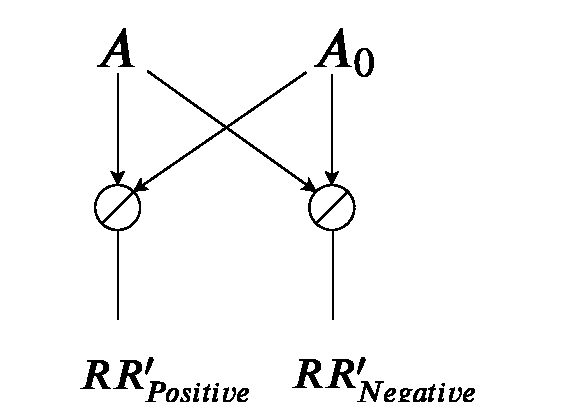
\includegraphics[width=0.5\textwidth]{figures/image_program_flow.pdf}
    \caption{Image visualization process flow}
    \label{fig:image_visualization_program_flow}
\end{figure}


\subsection{Spectrum processing}
\label{sec:spectrum_processing}

\begin{figure}[h]
    \centering
    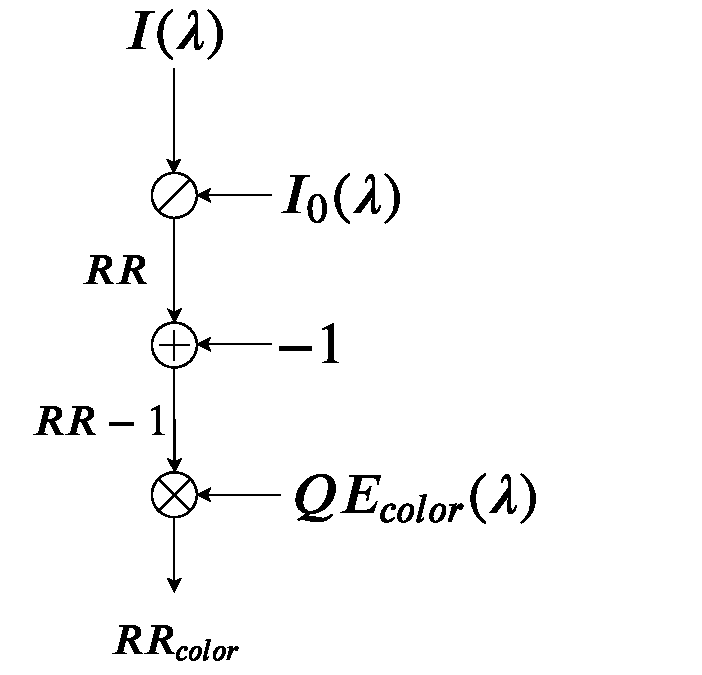
\includegraphics[width=0.5\textwidth]{figures/thesis_program_flow.pdf}
    \caption{Spectrum process flow}
    \label{fig:spectrum_process_flow}
\end{figure}

\subsection{Correlating Spectrometer to Camera}
\label{sec:method_correlating_spectrum_to_camera}
To get an idea of how well calibrated the camera is to the spectrometer and vice versa I propose the following calculation: 
Take the spatial average across the image from the camera and divide it with the spectral average of the spectrometer. 

\begin{equation}
    \label{eq:correlating_spectrum_to_camera}
    K = \frac{\mean{\vec{p}}}{\mean{RR}}
\end{equation}

This process is shown in figure \ref{fig:correlating_spectrum_and_image}.

\begin{figure}[h]
    \centering
    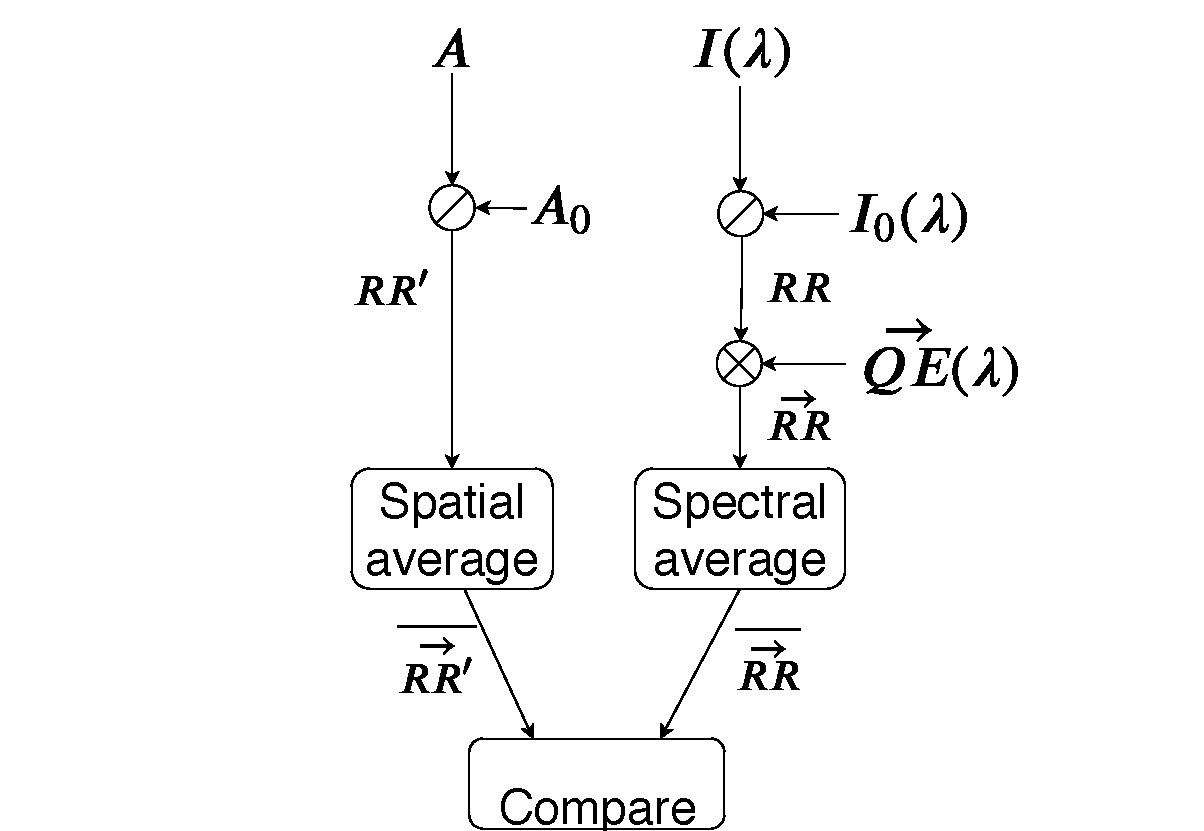
\includegraphics[width=0.75\textwidth]{figures/image_comparison_with_spectrometer.pdf}
    \caption{Correlating value between image and spectrum}
    \label{fig:correlating_spectrum_and_image}
\end{figure}


\subsection{Light}
Light is a crucial part of this project, as it is the source of input for both the camera and the spectrometer. It's also the link between the two sensors. The choosing of a sensor that can support both sensor types is therefore paramount. The camera is less selective on the spectral properties of the light source as it only requires a light source that is approximately white, i.e. have similar amounts of red, green and blue "wavelengths". It is however more selective in the spatial region as it can arise more problems for the camera if the lighting creates a lot of shadows or local problems like strong specular reflection making the pixel go into saturation. As implied the spectral properties of the light is more important for the spectrometer. For the spectrometer we want the spectrum to be as flat as possible. 

The characterization of the light source will be based on considerations from \cite{martinPracticalGuideMachine}, but also unfortunately be limited by available sources at the lab. % This paper provides a longer checklist, that can be simplified greatly under the following conditions: Stationary objects,


\section{Experimental setup}
The photos and spectrums where taken inside a lab with no external lights, and the real setup is as shown in figure \ref{fig:picture_of_setup_unlit}. %TODO: Change this figure into the side by side, lit - unlit

\begin{figure}[h]
    \centering
    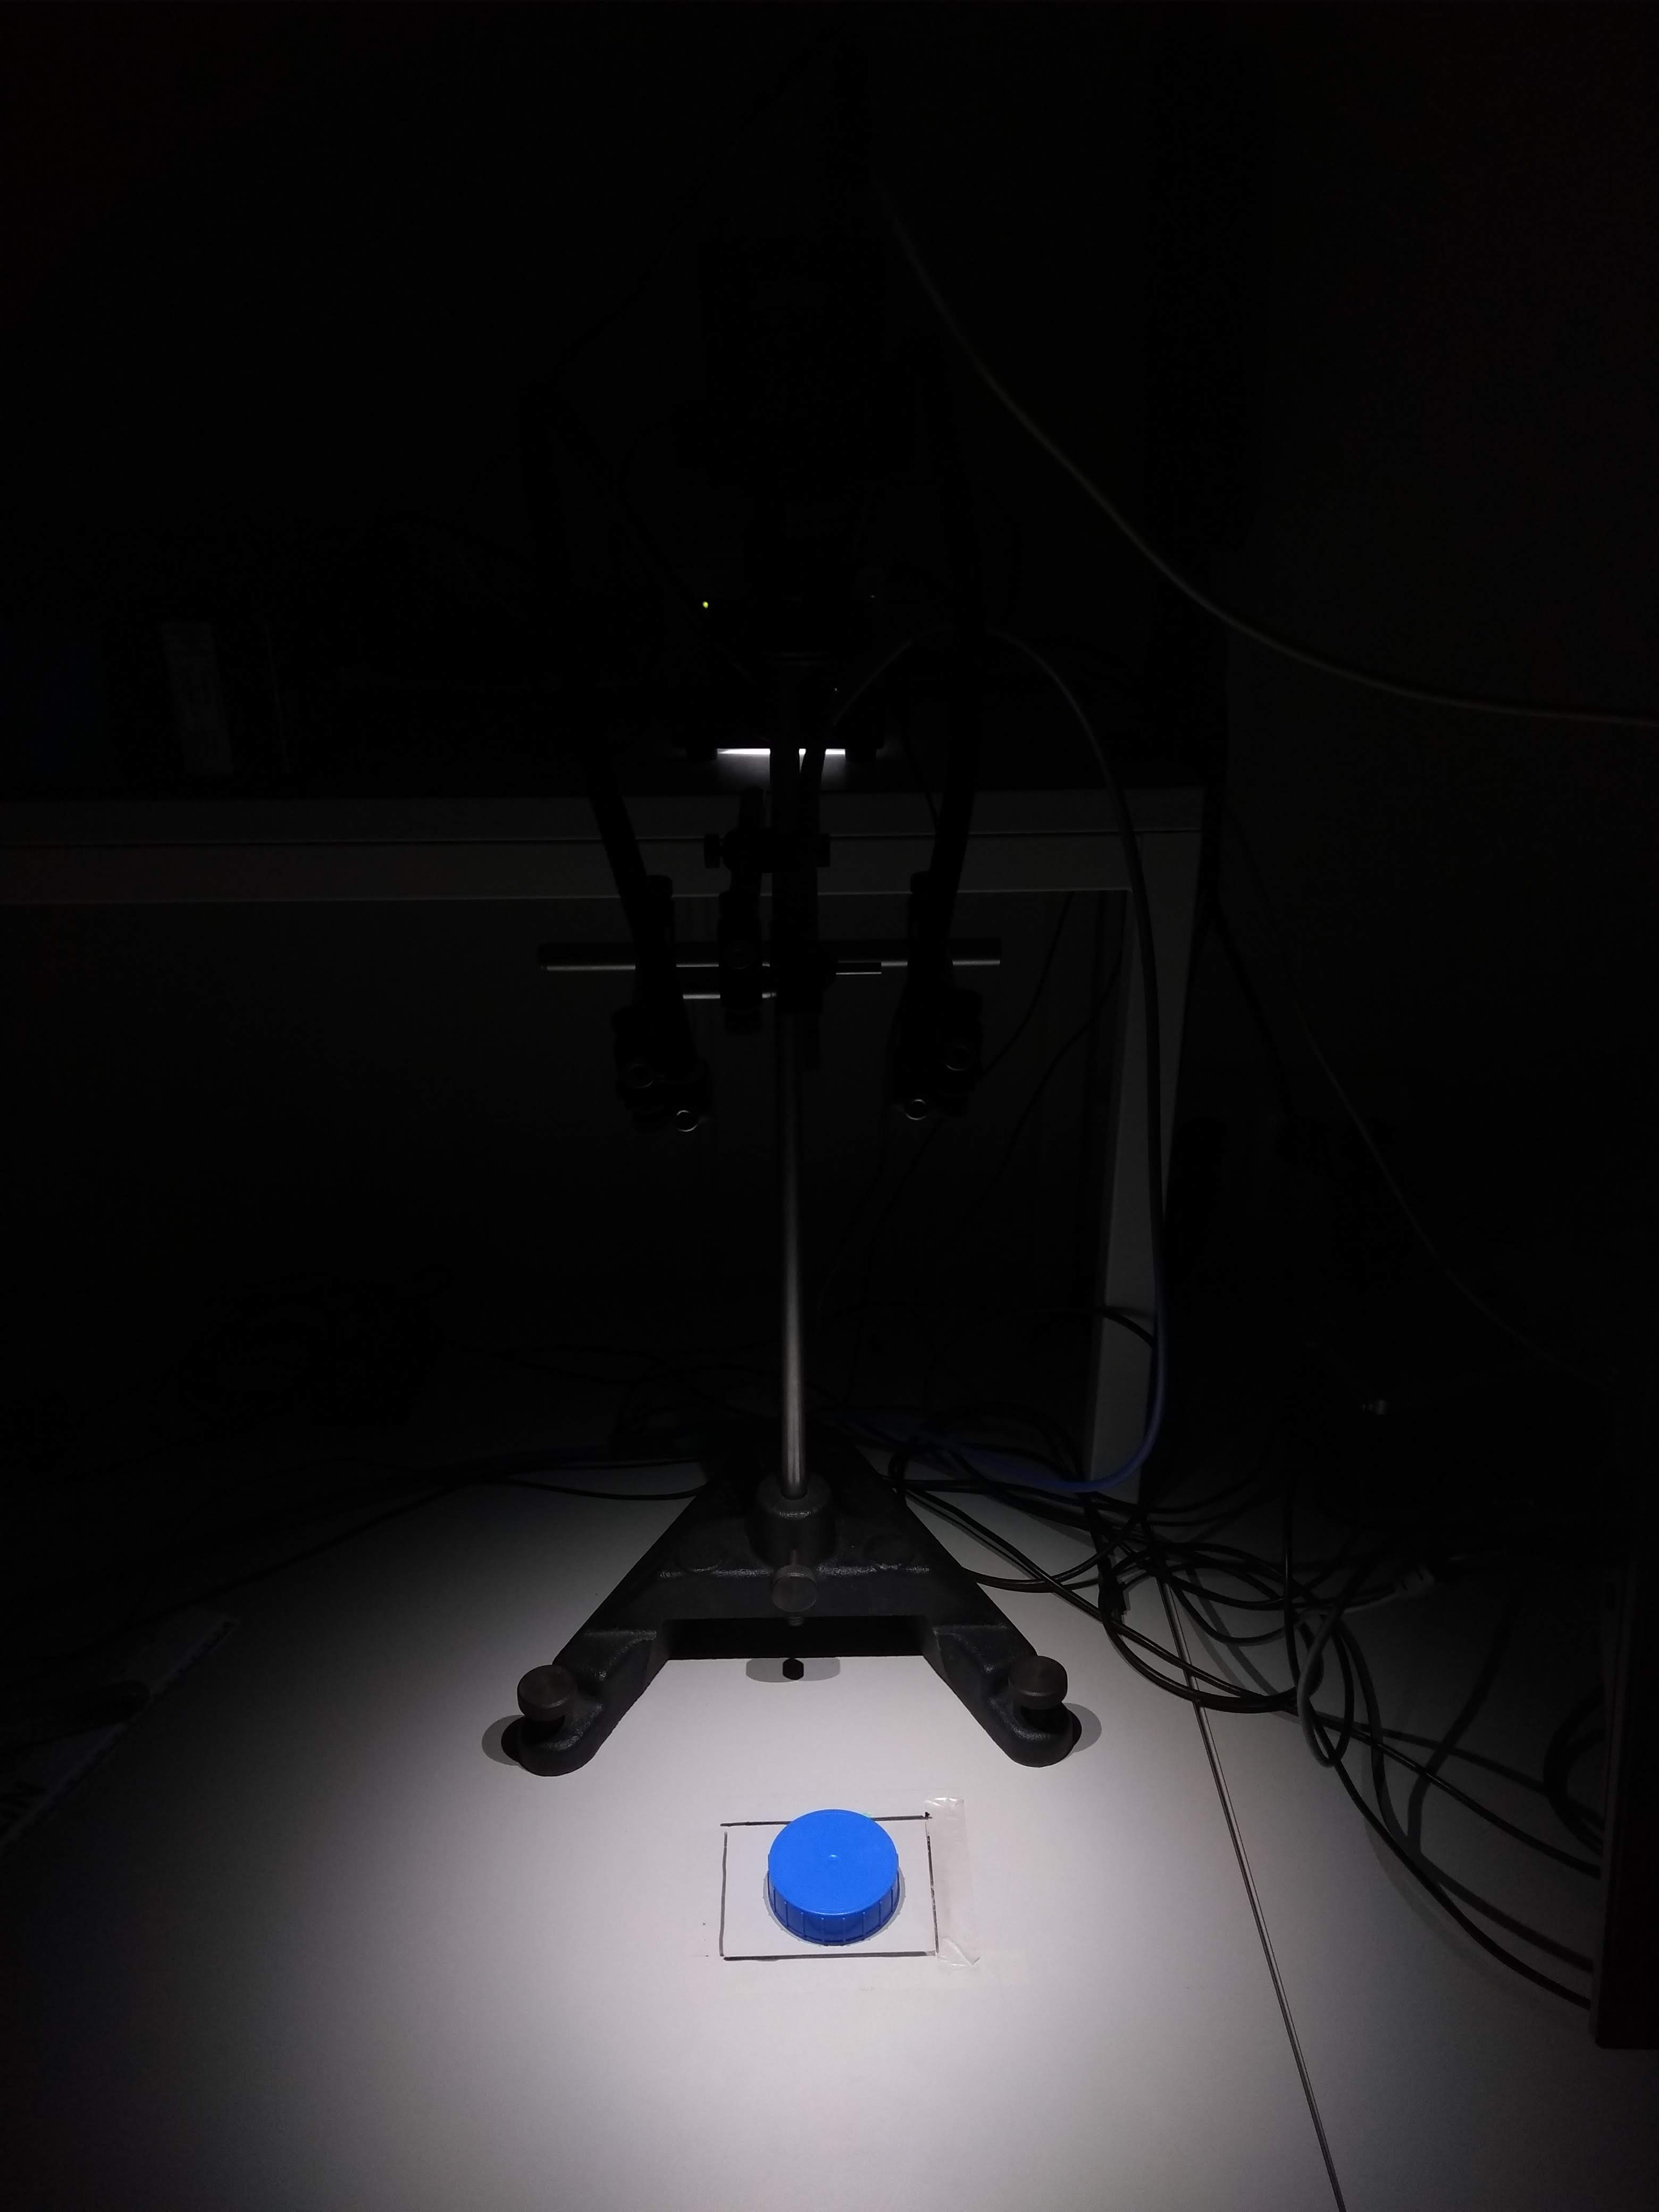
\includegraphics[width=0.3\textwidth]{figures/picture_taking_in_the_dark}
    \caption{Photo of the setup unlit}
    \label{fig:picture_of_setup_unlit}
\end{figure}

\subsection{Image processing}

To show how the processing was done, two images will be used as examples. One will be used as the reference image (figure \ref{fig:001_background}), and the other will contain an object to be analysed (figure \ref{fig:002_blue_cap}). These two images will then be sent through the process in figure \ref{fig:image_visualization_program_flow} with a noise limit of 10. 

The results from the processing are the two images in figure \ref{fig:hadamard_division_blue_cap}. They have been normalized and multiplied with 255 so that it is easy to see the changes. %TODO Are they actually histogram equalized? I don't really think so, I just normalized them and multiplied with 255.
Figure \ref{fig:002_blue_cap_positive_difference} shows what colors in what pixels have gotten more light after the blue cap was introduced. On the other hand figure \ref{fig:002_blue_cap_negative_difference} shows the colors that have gotten weaker after introducing the cap. What this means will be discussed further in section \ref{sec:blue_cap_discussion}

\begin{figure}[h]
    \begin{subfigure}{0.5\textwidth}
        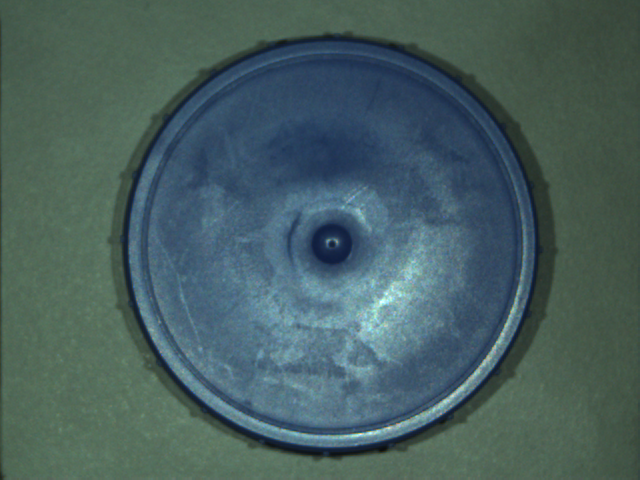
\includegraphics[width=0.9\linewidth, height=5cm]{figures/camera_pictures_png/002_blue_cap.png}
        \caption{002 Blue cap, $A$}
        \label{fig:002_blue_cap}
    \end{subfigure}%
    \begin{subfigure}{0.5\textwidth}
        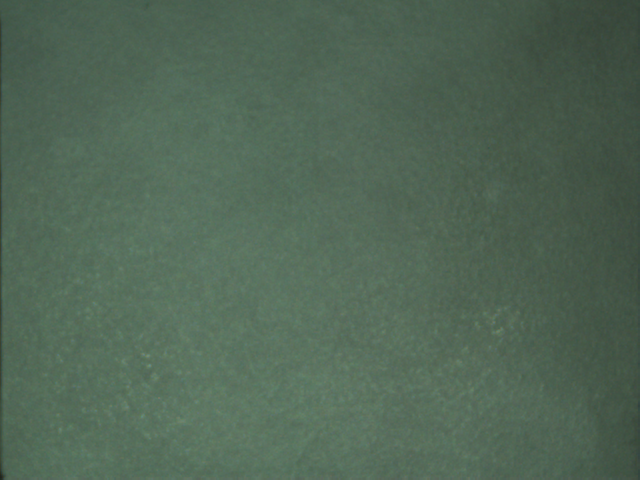
\includegraphics[width=0.9\linewidth, height=5cm]{figures/camera_pictures_png/001_background.png}
        \caption{001 Background, $A_0$}
        \label{fig:001_background}
    \end{subfigure}
    
    \caption{The original images being used in figure \ref{fig:hadamard_division_blue_cap}}
    \label{fig:blue_cap_and_background}
\end{figure}

\begin{figure}[h]
        \begin{subfigure}{0.5\textwidth}
            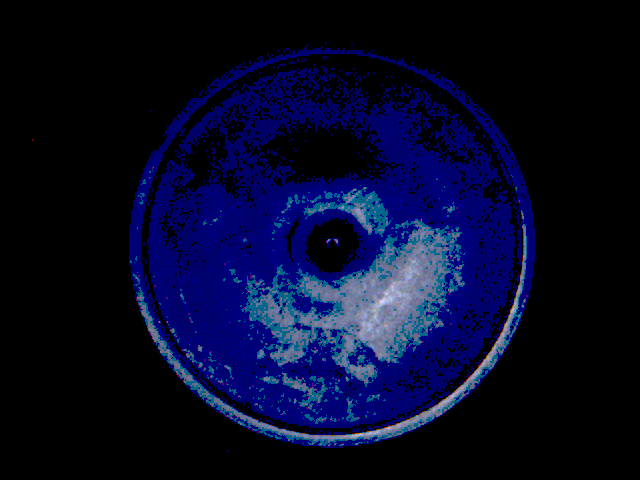
\includegraphics[width=0.9\linewidth, height=5cm]{figures/processed_camera_pictures/002_blue_cap_positive_difference.png}
            \caption{$RR'_{positive}$}
            \label{fig:002_blue_cap_positive_difference}
        \end{subfigure}%
        \begin{subfigure}{0.5\textwidth}
            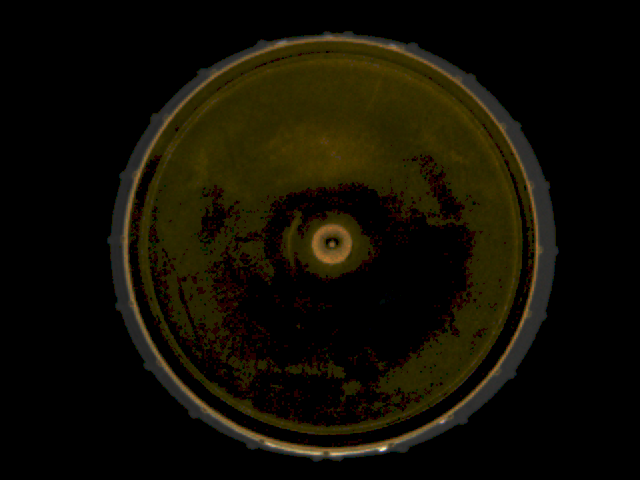
\includegraphics[width=0.9\linewidth, height=5cm]{figures/processed_camera_pictures/002_blue_cap_negative_difference.png} 
            \caption{$RR'_{negative}$}
            \label{fig:002_blue_cap_negative_difference}
    \end{subfigure}
    
    \caption{Hadamard division for the blue cap}
    \label{fig:hadamard_division_blue_cap}
\end{figure}

\subsection{Spectrum processing}

The spectrum was analysed in a similar manner, but here it was not necessary for the sake of visualization to split it into two results. It was however needed to subtract 1 from the results so that it was easy to compare the spectrums before and after multiplying with QE to each other. It also helped for comparison with the image. 
The recorded spectrums for the reference image and the blue cap is shown in figure \ref{fig:blue_cap_and_reference_spectrum}. The black line is the reference background spectrum, and the blue line is the line when the blue cap is introduced. 

\begin{figure}[h]
    \centering
    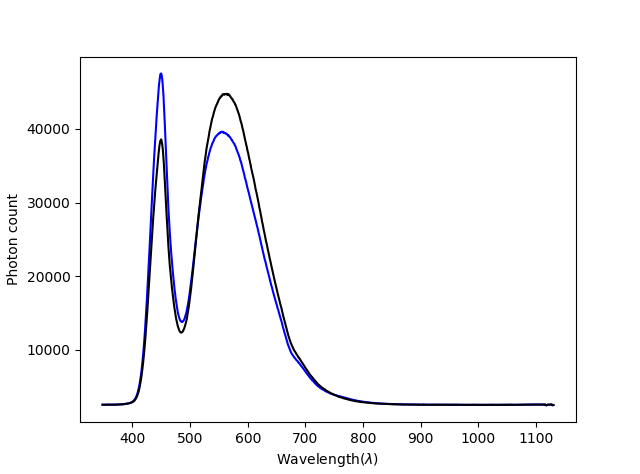
\includegraphics[width=0.75\textwidth]{Plots/blue_cap_original_spectrum_and_background.png}
    \caption{Comparison of blue cap (blue) and reference specter (black)}
    \label{fig:blue_cap_and_reference_spectrum}
\end{figure}


Figure \ref{fig:blue_cap_spectrum} shows relative reflectance minus one for the blue cap. It also includes the spectrums that the camera "sees" for each color, i.e. the wavelength parts and their respective magnitudes that is taken in by the CCD sensor. They are shown in their original colors; blue, green and red. The quantum efficiency used is shown in figure \ref{fig:quantum_efficiency_camera} in the appendix. 

\begin{figure}[h]
    \centering
    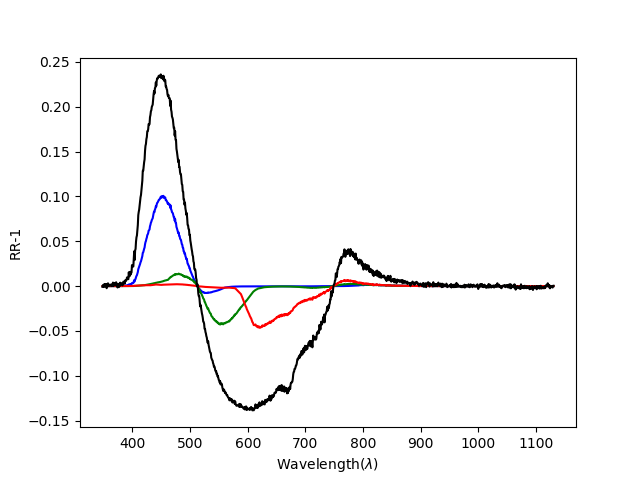
\includegraphics[width=0.75\textwidth]{Plots/blue_cap_rr_minus_one_with_qe.png}    
    \caption{Spectrum of blue cap}
    \label{fig:blue_cap_spectrum}
\end{figure}


\subsection{Discussion of processing}

\subsection{Blue cap}
\label{sec:blue_cap_discussion}
The picture of the blue cap will be used as a basement for discussion about the image processing. 

Figure \ref{fig:002_blue_cap_positive_difference} shows what colors in what pixels have gotten more light after the blue cap was introduced. It is of no surprise that blue is the dominant here, but there are also some spots that have a strong white color. This is due to the difference between specular and diffusive reflection introduced in section \ref{sec:theory_reflection}. 

Specular reflection reflects in the same direction and will for that reason give a stronger signal than diffusive where it hits. It will however only hit if the angle between the light source, the object and the camera is just so. It is because of the strong reflection that it appears white, all three of the color sensors have reached their limit and is given out the maximum value. Specular reflection will only appear in the $RR'_{positive}$ image. 

For more diffusive parts however the light is spread in several directions and the return value to the camera is therefore weaker and it is not normal to over expose these reflections. Diffusive reflectance shows up in both $RR'_{positive}$ and $RR'_{negative}$. It is what gives us the most color to work with. 


\subsection{Spectrum of camera}

\subsection{Correlating Spectrometer to Camera}

After processing the images and spectrum as shown in figure \ref{fig:correlating_spectrum_and_image} 

\section{Results}

\subsection{Ideal situation}
\label{sec:ideal_situation}
30 images and spectrums where run through the software and the average value was compared to each other. The spatial and spectral averages are plotted against each other in figure \ref{fig:spectral_vs_spatial_values} together with three linear regression lines, one for each color. 


\begin{figure}[h]
    \centering
    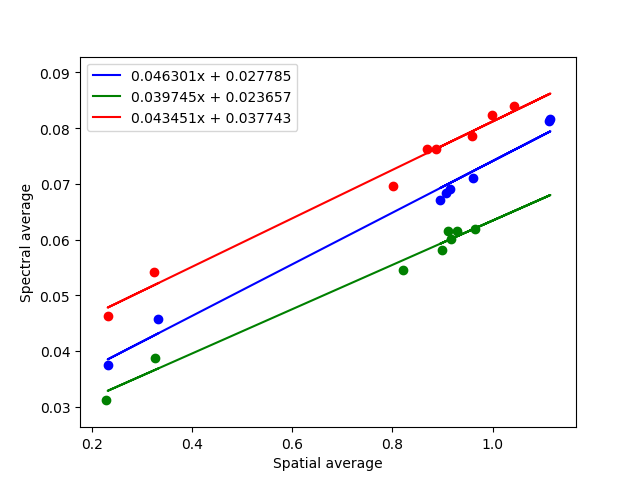
\includegraphics[width=0.75\textwidth]{Plots/spectral_vs_spatial_average_with_regression.png}
    \caption{Spatial and spectral averages plotted against each other with the fitted regression lines}
    \label{fig:spectral_vs_spatial_values}
\end{figure}

\subsection{Pertubation}
To see how well the value can be used for testing correspondence between image and spectrum, several images where taken that show non-ideal situations. These images will be compared to the regression lines created in section \ref{sec:ideal_situation} with the error function. These images are made with 10 randomly chosen settings from the ideal case, but with some unideal pertubation. 

For both the ideal and unideal cases the average error and variance of the error compared to the regression line was calculated and is presented in \ref{tb:error_estimate}.

\begin{table}[h]
    \centering
    \caption{Estimated error of the regression lines}
    \label{tb:error_estimate}
    \begin{tabular}{@{}llllllll@{}}
    \toprule
                   &                 & \multicolumn{3}{l}{Error average} & \multicolumn{3}{l}{Error variance} \\ \midrule
    Situation      & \#              & Blue       & Green     & Red      & Blue       & Green     & Red       \\
    Ideal          & 30              & 0.001261   & 0.001229  & 0.001370 & 6.744e-07  & 5.384e-07 & 8.963e-07 \\
    Ambient light  & 10              & 0.001805   & 0.001544  & 0.002349 & 1.860e-06  & 2.488e-06 & 1.016e-06 \\
    Border object  & 10              & 0.0007057  & 0.0005739 & 0.001615 & 6.581e-07  & 2.114e-07 & 6.382e-07 \\
    Outside object & 10              & 0.0006382  & 0.0009339 & 0.002476 & 1.174e-07  & 1.430e-07 & 1.876e-07 \\ \bottomrule
    \end{tabular}
\end{table}


\textbf{Ambient light}
These images where taken without turning of the light in the room. And with a fluorescent stand lamp on pointing towards the measurement area. Figure \ref{fig:ambient_light_plot} shows how these data points compare to the regression lines made in the ideal situation.

\begin{figure}[h]
    \centering
    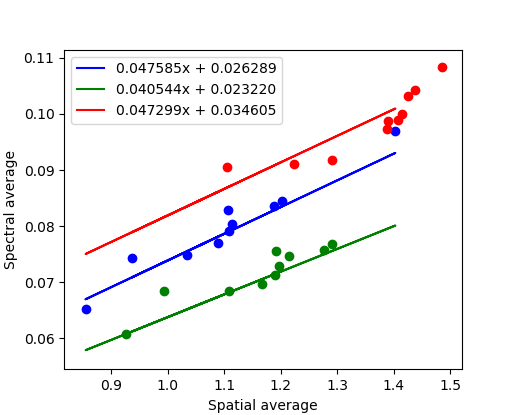
\includegraphics[width=0.5\textwidth]{Plots/spectral_vs_spatial_average_with_regression_ambient_light.png}
    \caption{Ambient light data points compared to ideal regression line}
    \label{fig:ambient_light_plot}
\end{figure}

\textbf{Border of imaging area}
Objects where put so that they where only partly inside the imaging area, but could still be seen by the spectrometer. Figure \ref{fig:boundary_objects_plot} shows how these data points compare to the regression lines made in the ideal situation.

\begin{figure}[h]
    \centering
    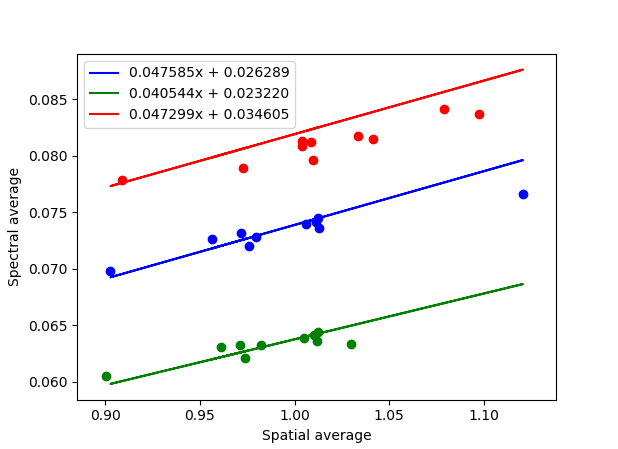
\includegraphics[width=0.5\textwidth]{Plots/spectral_vs_spatial_average_with_regression_boundary_objects.png}
    \caption{Objects placed on the boundary}
    \label{fig:boundary_objects_plot}
\end{figure}

\textbf{Outside the image area}
The same object where put inside the cameras viewpoint for every image, but a different object where put just outside it. It should still be inside the spectrometers view angle. Figure \ref{fig:outside_objects_plot} shows how these data points compare to the regression lines made in the ideal situation.

\begin{figure}[h]
    \centering
    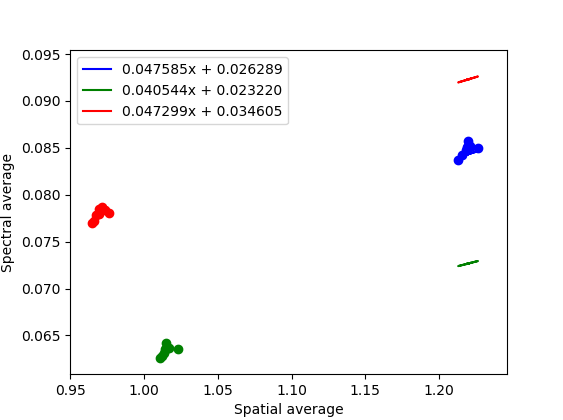
\includegraphics[width=0.5\textwidth]{Plots/spectral_vs_spatial_average_with_regression_outside_objects.png}
    \caption{One object inside boundary, another outside}
    \label{fig:outside_objects_plot}
\end{figure}

%\subsubsection{Specular reflection}

\section{Discussion}
The spatial and spectral average should be two sides of the same story, if the camera and the spectrometer are watching the same area and the conditions haven't changed between the camera taking the picture and the spectrometer taking the spectre. The purpose of taking these results where to test this postulate that was originally stated in section \ref{sec:introduction}.

Figure \ref{fig:spectral_vs_spatial_values} shows the results from 30 pictures taken under ideal conditions. The lines shown in blue, green and red are regression lines (sec \ref{sec:regression}) that are made as a minimum variance fit to the points. It looks like each of the color sensors have approximately the same number $a$, meaning that they have similar derivatives, but different $b$ means that they cross the y axis at different points. 

The error measurement given in table \ref{tb:error_estimate} shows the amount of error in the different situations. From the table we can see that the ambient light is the type of noise that is creating the most variance from the regression line. The other measurements actually show less variance which was not expected, but probably means that the acceptance cone of the spectrometer was smaller than expected, and not any bigger than the cameras acceptance cone. 

\textbf{Ambient light}
From the results it can be inferred that the light sources where the most important in this setup. Having ambient light on made the error increase to almost twice the previous error. This can be due to: 
\begin{itemize}
    \item More shadows are formed because light comes from other directions. 
    \item The reference picture without ambient light is very different to an image with ambient light. 
    \item The overhead lamp has many spikes in its spectrum, which could be a source of noise. 
\end{itemize}


\textbf{Border of the imaging area} and \textbf{Outside the image area}
Both of these led to smaller error than the ideal situation, which is strange. It can be due to the acceptance cone being much smaller than assumed, leading to changes outside of the black box not making any difference. This combined with the smaller change between image and reference due to the objects being placed on the border could explain the smaller error. 

\textbf{Shadows}
Part of the reason that parts of the wavelength gets weaker when an object is introduced is due to shadows. If the light doesn't come from the same fiber that is also receiving the light, an object with depth will cast a shadow. The image will get affected by this and in figure \ref{fig:002_blue_cap_negative_difference} you can see a darker white around the cork. Due to using two light sources it doesn't become a complete shadow. It should be possible to recognize the shadow with image processing and remove it. For the spectrum the shadow will decrease the amplitude of the resultant spectrum, but since the shadow effectively means that the light intensity is halved for all wavelengths this shouldn't affect the form of the spectrum. The reason it should be halved is that in our images one of the two light sources have always been able to light up every point. A shadow in this case is therefore when one light source is blocked. With more heterogenous materials both light sources can be blocked. This will not be addressed here.



The effects of the dark current \ref{sec:noise_and_dark_current} was hopefully minimized by finding the relative reflectance and introducing the noise limit into the image processing. 

\section{Conclusion}

It is a clear correlation between spatial and spectral average which seems to follow the regression lines well. There is however an amount of error that makes it hard to use for determining if the image and spectrum is perfectly of the same object. It is very good for finding out if there is to much noise from the ambient light. It seems like the test was lacking somewhat in diversity.

\bibliographystyle{plain}
\bibliography{references.bib}

\section{Appendix}


\subsection{Code}
\label{sec:appendix_code}
All the code used in this project is contained within one file. The main function has all the program flow, while the functions introduced above are written in a functional programing manner. 

Code used in this project: 

\lstinputlisting[language=Python]{image_and_spectrum_analyzis.py}

\subsection{Plots not included in the report}
\label{sec:appendix_plots}

%Figure \ref{fig:quantum_efficiency_camera} shows the quantum efficiency of the Bayer mask in the cameras CCD sensor. 
%\begin{figure}[h]
%    \centering
%    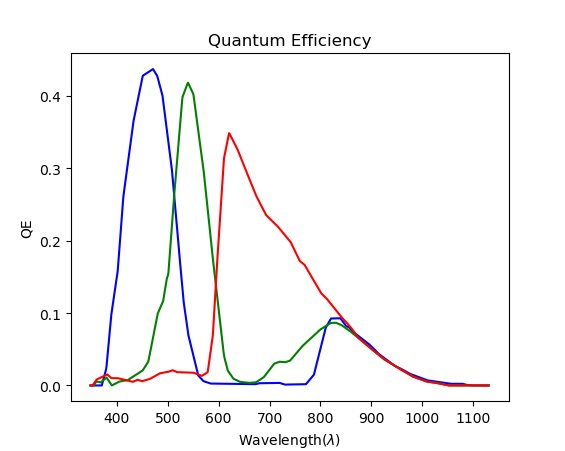
\includegraphics[width=1\textwidth]{Plots/quantum_effiency.png}
%    \caption{The quantum efficiency of the camera}
%    \label{fig:quantum_efficiency_camera}
%\end{figure}


Figure \ref{fig:relative_reflection_around_zero} shows $RR-1$ for nine of the objects being analyzed. 
%TODO3 Figure \ref{fig:relative_reflection_around_zero} shows nine plots, the first one shows the reference spectrum, the spectrum without any objects. The following eight plots shows the Relative Reflectance (\ref{eq:relative_reflectance}), their 
\begin{landscape}
\begin{figure}[t]
    \centering
    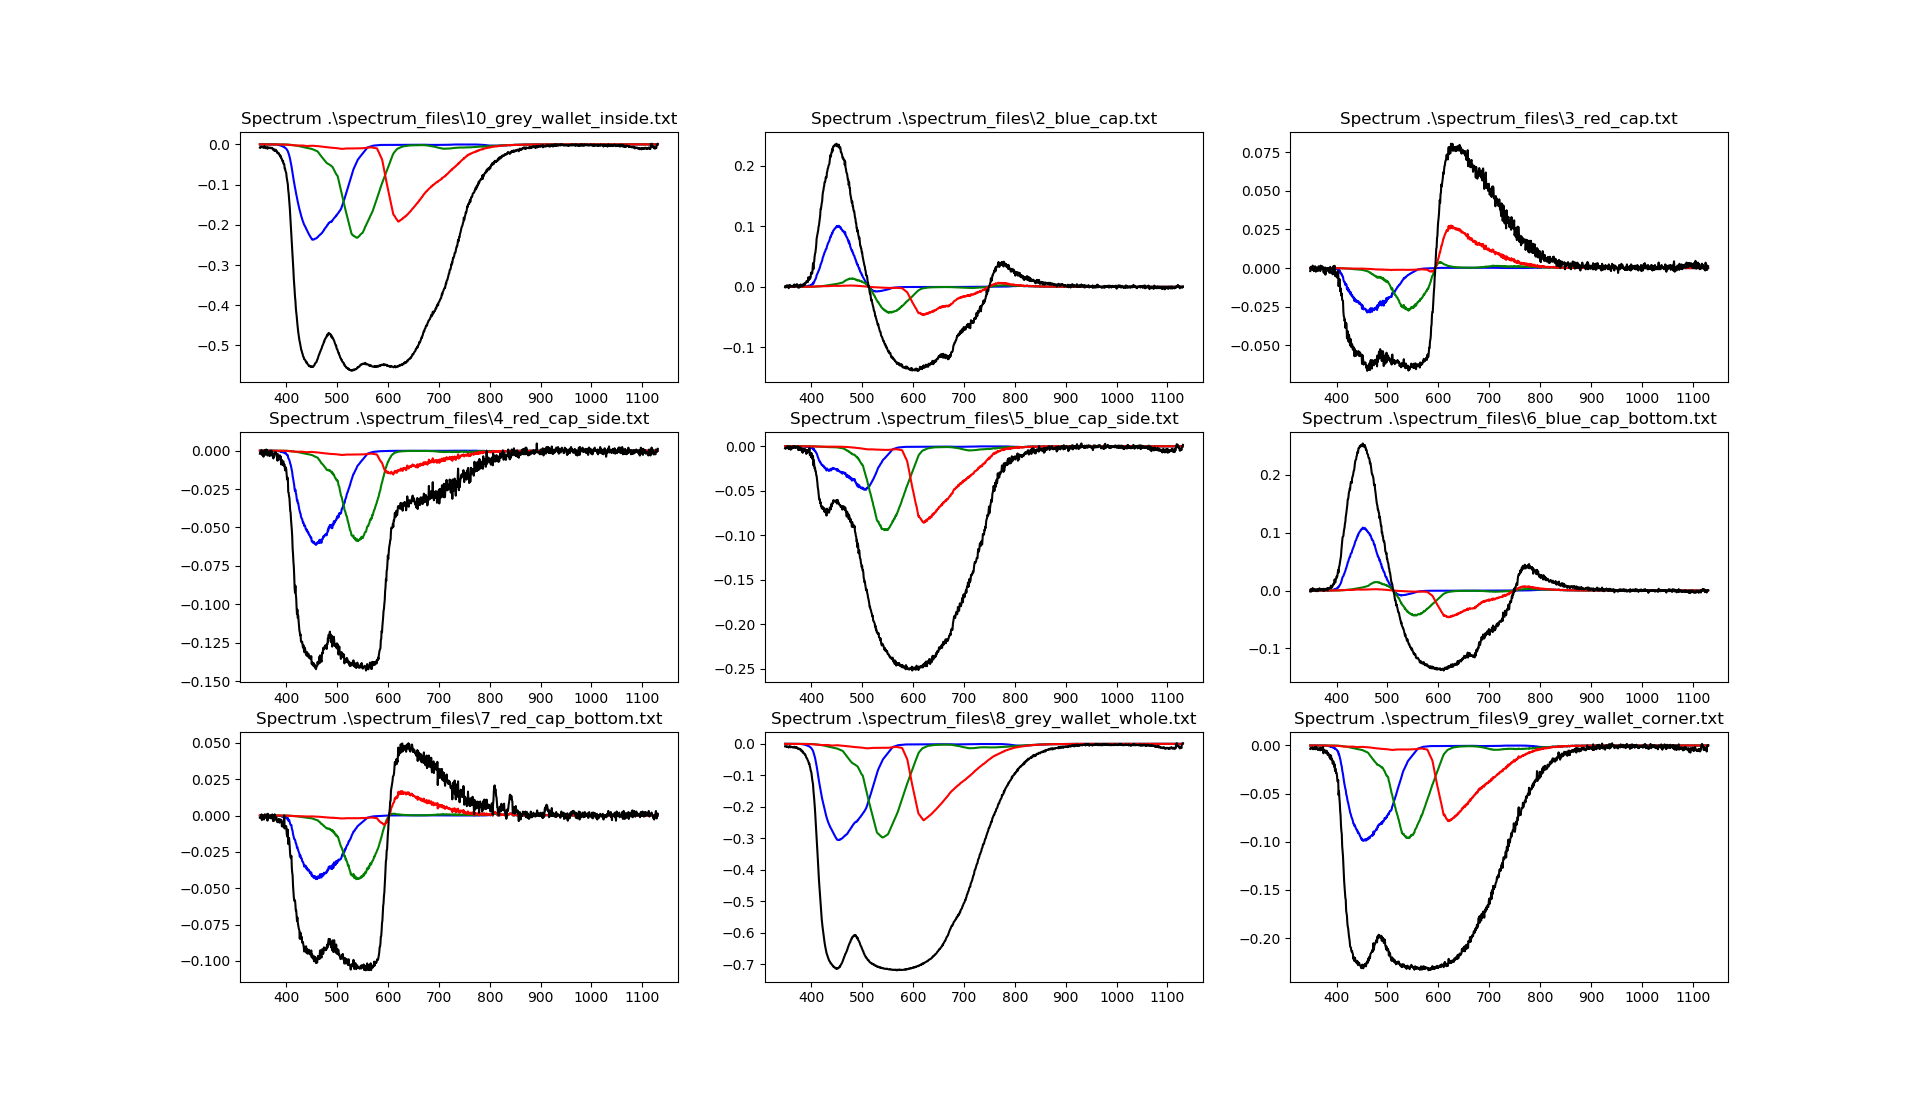
\includegraphics[width=1\paperwidth]{Plots/relative_reflectance_around_zero_with_qe_color_response.png}
    \caption{Relative reflection centered around zero}
    \label{fig:relative_reflection_around_zero}
\end{figure}
\end{landscape}




\end{document}